\documentclass{article}

\usepackage{graphicx}
\usepackage{tikz}
\usepackage{tikzsymbols}
\usetikzlibrary{calc,patterns,shapes.geometric}
\pagestyle{empty}
\usepackage[margin=0pt]{geometry}
\geometry{papersize={14in,12in}}

\def\centerarc[#1](#2)(#3:#4:#5){\draw[#1] ($(#2)+({#5*cos(#3)},{#5*sin(#3)})$) arc (#3:#4:#5);}

\begin{document}
	\begin{figure}
		\centering
		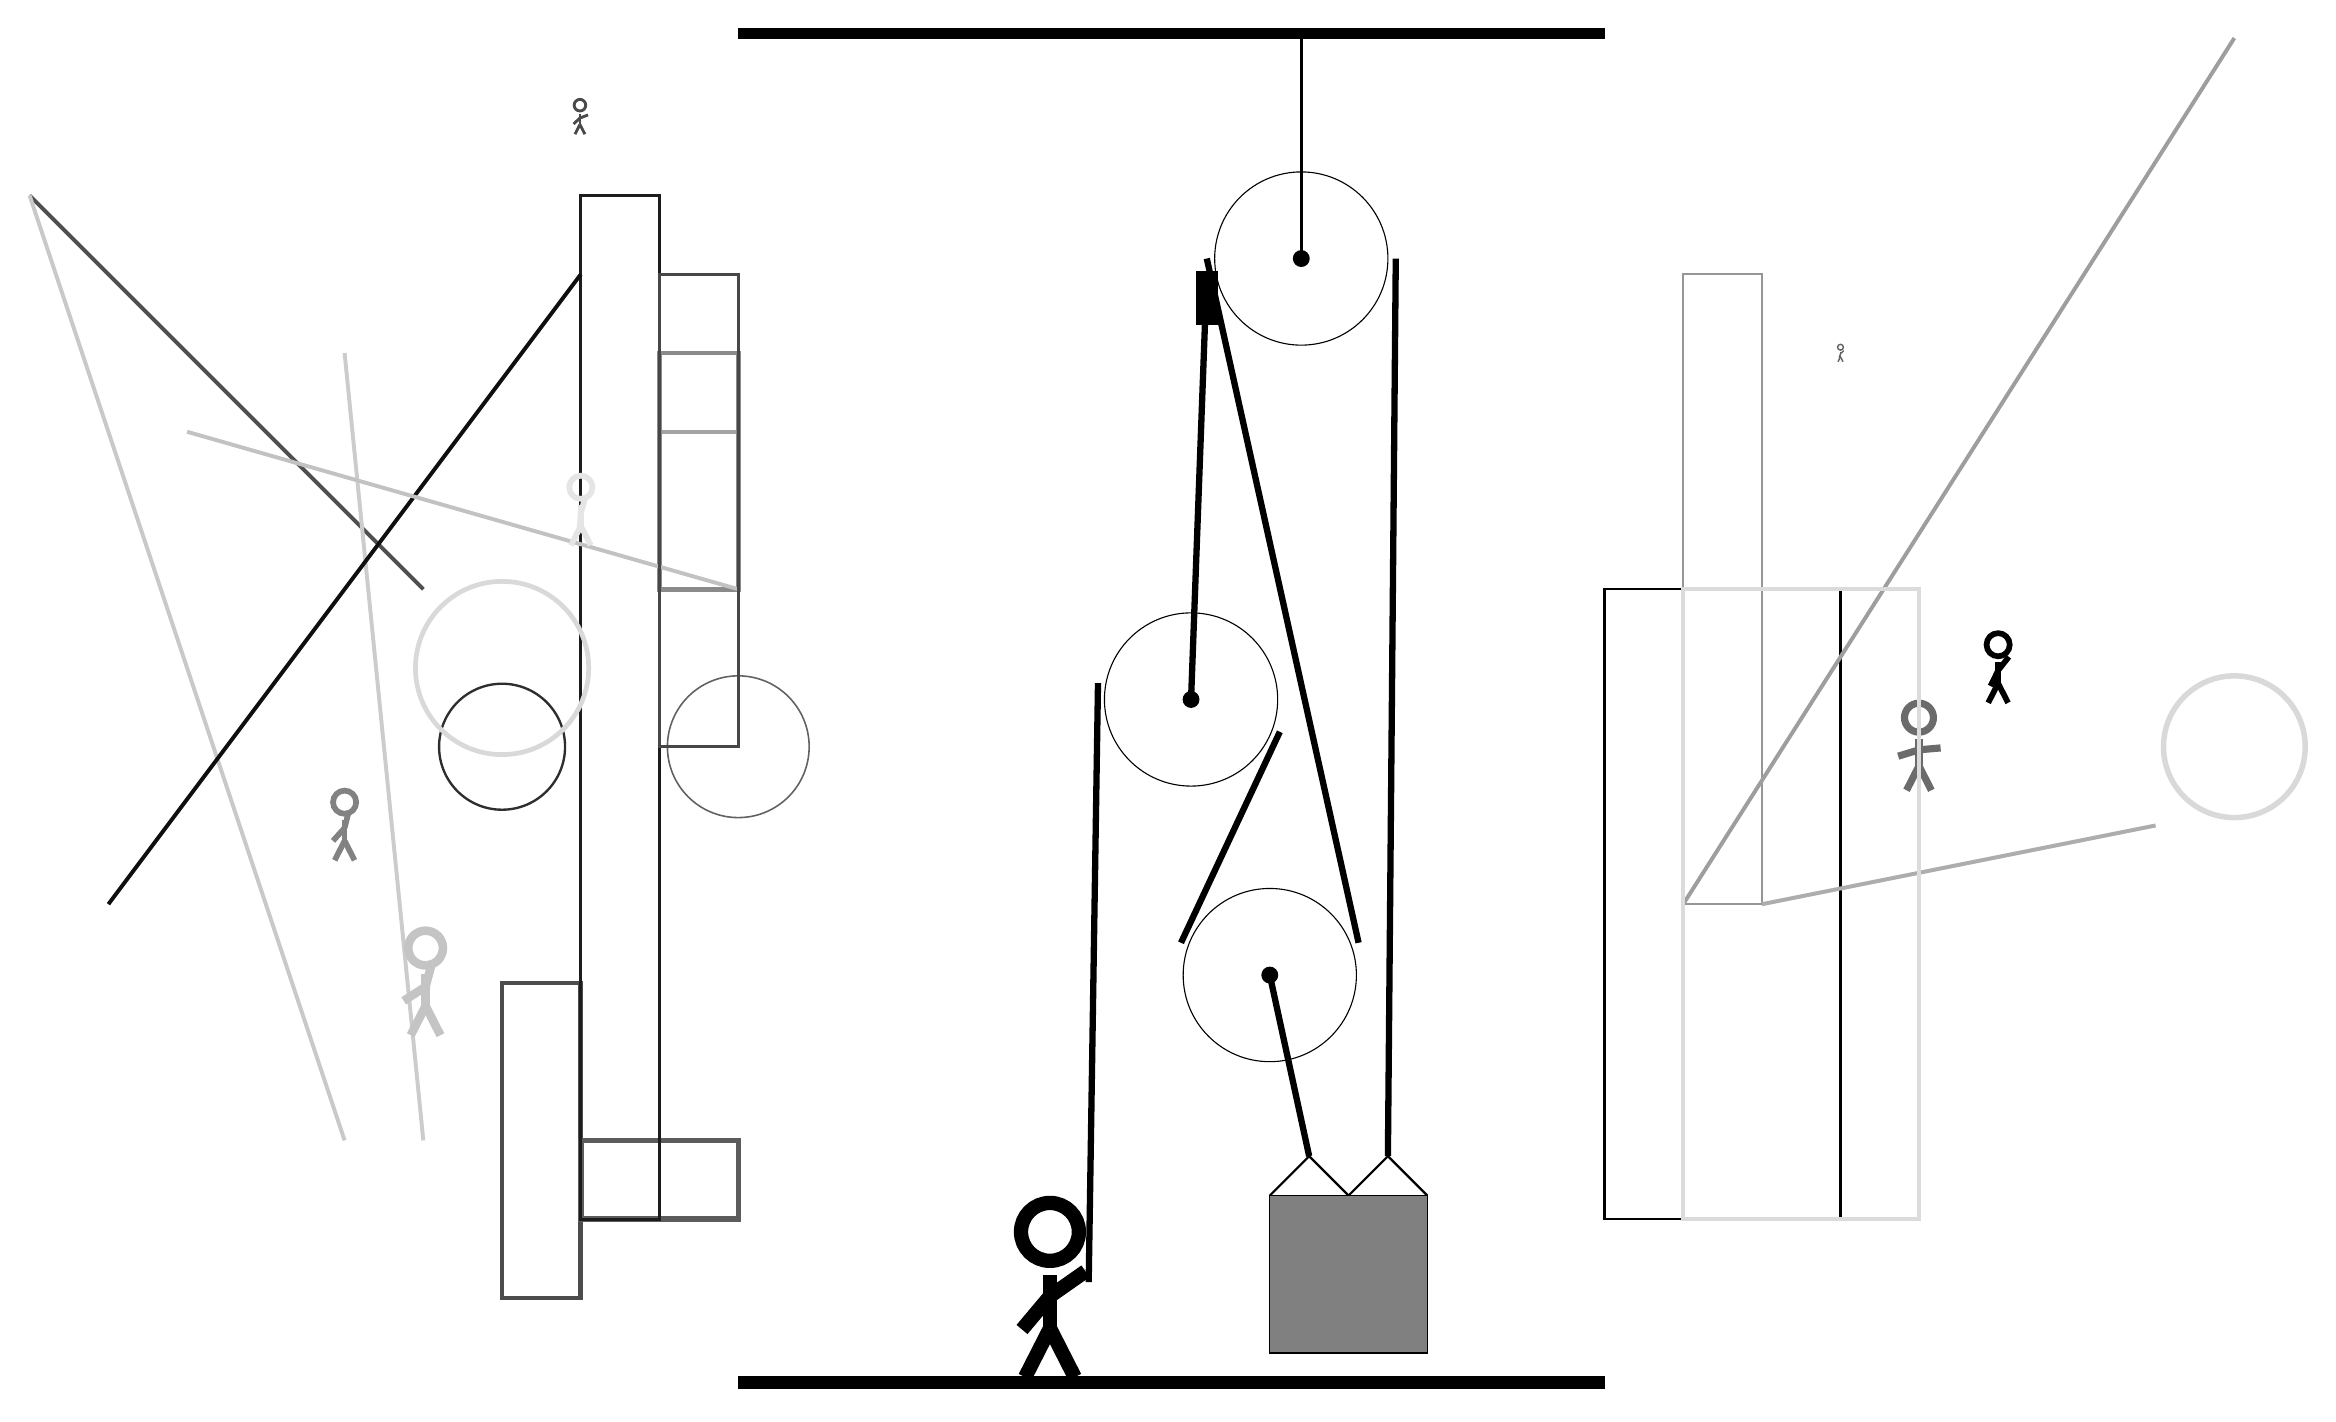
\begin{tikzpicture}
			%%%%% START %%%%%
			
			\draw[fill=black] (-6, 14) rectangle (5, 14.125);
			
			\draw (-0.25, 5.6) circle (1.1);
			\draw[fill=black] (-0.25, 5.6) circle (0.1);
			
			\draw[line width=0.2mm, color=black!41] (6, 3) rectangle (7, 11);
			
			\node[line width=0.5mm, color=black!49] at (-11, 4) {\Strichmaxerl[4][48][76]};
			\draw [line width=0.3mm, color=black!82](-9, 5) circle (0.8);
			\draw[line width=0.3mm, color=black!100] (5, 7) rectangle (8, -1);
			\draw[line width=0.5mm, color=black!32](7, 3) -- (12, 4);
			\node[line width=0.3mm, color=black!58] at (9, 5) {\Strichmaxerl[5][17][5]};
			\draw[line width=0.5mm, color=black!38](6, 3) -- (13, 14);
			\draw[line width=0.6mm, color=black!70] (-8, 2) rectangle (-9, -2);
			\draw[line width=0.5mm, color=black!36] (-6, 7) rectangle (-7, 9);
			\draw[line width=0.5mm, color=black!69](-10, 7) -- (-15, 12);
			\node[line width=0.6mm, color=black!100] at (10, 6) {\Strichmaxerl[4][64][52]};
			\draw[line width=0.5mm, color=black!21](-11, 0) -- (-15, 12);
			\draw[line width=0.5mm, color=black!20](-10, 0) -- (-11, 10);
			\node[line width=0.7mm, color=black!71] at (-8, 13) {\Strichmaxerl[2][43][21]};
			\draw[line width=0.7mm, color=black!64] (-6, 0) rectangle (-8, -1);
			\draw [line width=0.2mm, color=black!62](-6, 5) circle (0.9);
			
			\node[line width=0.3mm, color=black!61] at (8, 10) {\Strichmaxerl[1][73][42]};
			\draw[line width=0.4mm, color=black!89] (-8, -1) rectangle (-7, 12);
			\draw [line width=0.6mm, color=black!15](-9, 6) circle (1.1);
			\draw [line width=0.7mm, color=black!15](13, 5) circle (0.9);
			\node[line width=0.6mm, color=black!23] at (-10, 2) {\Strichmaxerl[6][33][75]};
			
			\draw[line width=0.5mm, color=black!94](-8, 11) -- (-14, 3);
			\draw [line width=0.3mm, color=black!91](-11, 6) circle (0.0);
			\draw[line width=0.6mm, color=black!46] (-7, 7) rectangle (-6, 10);
			\draw[line width=0.5mm, color=black!24](-6, 7) -- (-13, 9);
			
			\draw[line width=0.5mm, color=black!14] (6, 7) rectangle (9, -1);
			
			\node[line width=0.4mm, color=black!10] at (-8, 8) {\Strichmaxerl[4][85][74]};
			\draw[line width=0.4mm, color=black!72] (-6, 5) rectangle (-7, 11);
			
			\draw (0.75, 2.1) circle (1.1);
			\draw[fill=black] (0.75, 2.1) circle (0.1);
			
			\draw (1.15, 11.2) circle (1.1);
			\draw[fill=black] (1.15, 11.2) circle (0.1);
			\draw[very thick] (1.15, 11.2) -- (1.15, 14);
			
			\draw[thick]  (0.75, -0.7) -- (1.25, -0.2) -- (1.75, -0.7) -- (2.25, -0.2) -- (2.75, -0.7);
			\draw[fill=black!50] (0.75, -0.7) rectangle (2.75, -2.7);
			
			\draw[line width=0.8mm] (-0.25, 5.6) -- (-0.05, 11.0);
			\draw[line width=0.8mm, fill=black](-0.15, 10.4) rectangle (0.05, 11.0);
			\draw[line width=0.8mm] (-1.55, -1.8) -- (-1.4318, 5.8083);
			\centerarc[line width=0.8mm](-0.25, 5.6)(-20:170:1.2000000000000002);
			\draw[line width=0.8mm] (0.8776, 5.1896) -- (-0.3776, 2.5104);
			\centerarc[line width=0.8mm](0.75, 2.1)(160:380:1.2000000000000002);
			\draw[line width=0.8mm] (1.8776, 2.5104) -- (-0.05, 11.2);
			\draw[line width=0.8mm](0.75, 2.1) -- (1.25, -0.2);
			\centerarc[line width=0.8mm](1.15, 11.2)(0:180:1.2000000000000002);
			\draw[line width=0.8mm] (2.35, 11.2) -- (2.25, -0.2);
			
			\node at (-2, -1.9) {\Strichmaxerl[10][50][35]};
			
			\draw[fill=black] (-6, -3) rectangle (5, -3.15);
			
			%%%%% END %%%%%
		\end{tikzpicture}
	\end{figure}	
\end{document}